\documentclass[a4paper,11pt]{article}

%%%%%%%%%%%%%%%%%%%%%%%%%%%%%%%%%
%            ATENÇÃO            %
% NÃO ALTERE AS LINHAS A SEGUIR %
%%%%%%%%%%%%%%%%%%%%%%%%%%%%%%%%%

\usepackage[english]{babel}
\usepackage{float,graphicx,graphics,amssymb,amsfonts,newlfont,indentfirst}
\usepackage[centertags]{amsmath}
\usepackage{fancyhdr}
\usepackage{ragged2e}
\usepackage{geometry}
\geometry{top=0cm,bottom=2cm,left=3cm,right=2cm}
\usepackage[normalem]{ulem}
\pagestyle{fancy}
\usepackage{url}
\usepackage{color}
\usepackage[font+=small,leftmargin=4cm,rightmargin=0cm,indentfirst=false]{quoting}
%\fancyfoot{} %retira número das páginas do rodapé
\renewcommand{\rmdefault}{ptm}
\renewcommand{\sfdefault}{ptm}
\renewcommand{\ttdefault}{ptm}

\lhead{ERMAC, Volta Redonda -- RJ, 2023}

\fancypagestyle{capa}{%
	\fancyhead{}%
	\rhead{\textit{Trabalho apresentado no ERMAC, Volta Redonda -- RJ, 2023.}%
	\vspace*{11pt}}%
}

\usepackage{mathptmx} % Fonte Times em fórmulas

\headheight 10mm
\oddsidemargin 2.0mm
\evensidemargin 2.0mm
\topmargin -10mm
\textheight 240mm
\textwidth 160mm
\headsep 5mm
\parindent 1mm


%%%%%%%%%%%%%%%%%%%%%%%%%%%%%
% MODIFIQUE DAQUI EM DIANTE %
%%%%%%%%%%%%%%%%%%%%%%%%%%%%%

% pacotes adicionais
%\usepackage{algorithm}
\usepackage[pdftex]{hyperref} %permite resaltar texto
\hypersetup{colorlinks,citecolor=black,filecolor=black,linkcolor=black,urlcolor=black} %setup de hyperref
\bibliographystyle{unsrt}
\bibliographystyle{abntex2-alf}
\usepackage{etoolbox}
\patchcmd{\thebibliography}{\section*{\refname}}{}{}{}

\begin{document}

\centering{{\Large{\bf Tool for simulating tumor growth in various regions of the human body in three dimensions.}}

\begin{flushright}{\it
\vspace*{5mm}
Carlos Carret Miranda\\
University of Havana\\
carlos.carret@estudiantes.matcom.uh.cu

\vspace*{5mm}
\underline{ Reinaldo Rodríguez Ramos}\\
Department of Mathematics, Faculty of Mathematics and Computer Science, University of Havana, Cuba, and PPG-MCCT, Federal Fluminense University, Volta Redonda, Rio de Janeiro, Brazil.\\
reinaldo@matcom.uh.cu and reinaldorr@id.uff.br

\vspace*{5mm}
Panters Rodríguez Bermúdez\\
Departamento de Ciências Exatas, Universidade Federal Fluminense, Volta Redonda, Rio de Janeiro, Brazil\\
pantersrb@id.uff.br

% se necessário, adicione mais autores como nos blocos acima
}\end{flushright}


\setcounter{equation}{0} % NÃO modifique esta linha


\thispagestyle{capa}
\justifying{
{\noindent \bf Summary: }{\small{%
	%RESUMO 
 Cancer is a disease characterized by the uncontrolled growth of abnormal cells in the body. It is a complex and multifaceted disease that has challenged researchers and doctors for decades. The ability to visualize and understand tumor growth can provide valuable insights into how cancer develops and spreads, leading to significant improvements in cancer diagnosis, treatment, and prevention. The three-dimensional tumor growth simulation tool that is being developed is an important step in this direction. It allows for detailed visualization of tumor growth in different parts of the human body, which can provide valuable insights into how cancer develops and spreads. Additionally, the ability of this tool to simulate tumor growth in different parts of the body means that it can be used to study a wide range of cancer types. This tool utilizes a cellular automaton and a small-world network to create connections between cells, allowing for a more accurate representation of organ and tumor structures. Furthermore, it allows for the loading of configurations and parameters from external files, providing great flexibility to the tool and allowing for customization of the simulation to the specific needs of each case. For 3D rendering, the Marching Cubes technique is used, which enables detailed and accurate three-dimensional representation of tumors.
}}

\vskip 0.2cm  % NÃO modifique esta linha


{\small{ %PALAVRAS-CHAVE
\noindent{\bf{Keywords:}} Scientific Computing, Numerical Methods, and Applications. Cellular Automaton. Marching Cubes. 3D. Cancer. Tumor.
}}
}

%%%%%%%%%%%%%%%%%%%%%%%%%%%%%
%%%%%%%%%%%%%%%%%%%%%%%%%%%%%

\section*{Introduction}

The challenge of representing biological phenomena mathematically, physically, and computationally requires interdisciplinary synergy among experts in these fields. This collaboration enriches the traditional experimental method used in biological sciences by implementing mathematical models, which serve as tools to formulate and test hypotheses, guide experimental research, and refine the model based on the obtained results.~\cite{7}

Cancer is a disease that affects a large number of living organisms and is characterized by the presence of a group of abnormal cells that grow uncontrollably, disregarding the normal rules of cell division. It particularly affects humans, where its occurrence and development pose a threat to life. The malignancy of cancer varies and depends on factors such as the growth rate of cancer cells, their ability to spread to other tissues, and the possibility of recurrence after surgical removal.

The purpose of this type of research is to achieve a deeper understanding of biological processes through an iterative cycle of theory and experimentation. Additionally, mathematical models can be used to assist in the conception and design of therapeutic strategies, providing a more precise and personalized insight into the treatment of each patient.

In the case of this project, a cellular automaton and a small-world network are used to model the interactions between cells, providing a more accurate representation of tumor growth. The parameters and configurations can be loaded from external files, offering great flexibility in adapting the simulation to the specific needs of each case. The work being conducted is a part of a larger thesis project that is currently in progress. The project aims to simulate tumor growth in small organs and involves loading and utilizing parameters for the simulation. The graph of cells with their connections is visualized and analyzed, along with the visualization of the tumor size throughout the simulation. The focus of the next stages is to improve the existing implementation and incorporate changes based on details found in medical literature. Additionally, efficient algorithms will be implemented to process large amounts of cells and their connections. In the future, the project aims to incorporate Artificial Intelligence and Machine Learning techniques to achieve better approximations to reality.

The technique of Marching Cubes~\cite{5} is used for 3D rendering, providing a detailed and precise visualization of tumors. This visualization can provide valuable insight into how cancer develops and spreads, which can be essential for the development of effective therapies and treatments. By visualizing tumor growth in three dimensions, doctors and scientists can gain a better understanding of tumor evolution and how it may affect surrounding tissues. This information can be crucial for the development of effective therapies and treatments for cancer.


\section*{Submission}

\textbf{Cellular Automaton}

In this section, the cellular automaton model presented in this work is conceived. It begins by formally defining a cellular automaton~\cite{7}.

A cellular automaton is a tuple $(\mathcal{L}; \mathcal{N}; \mathcal{E}; \mathcal{R})$ composed of the following representative elements~\cite{2}:
\begin{itemize}
\item [$\mathcal{L}$:] t is a potentially infinite set of cells.
\item [$\mathcal{N}$:] $\mathcal{L} \times \mathcal{L} \rightarrow \lbrace 0,1 \rbrace$ is a neighborhood function, which can be seen as a relation, usually reflexive and symmetric, between cells. This function shows which pairs of cells are neighbors, that is, the geometry of the cellular organization.
\item [$\mathcal{E}$:] It is a set of states. Each cell in the set $\mathcal{L}$ is assigned an associated state at each time step.
\item [$\mathcal{R}$:] $\mathcal{E}^{|\mathcal{N}(v)|} \rightarrow \mathcal{E}$ is a locally defined transition function. This function is the core of the dynamics of a cellular automaton and is commonly expressed through rules that define the state of the cell in the next time step based on the state of the neighboring cells. The set containing the state of the neighboring cells is obtained through the function $\mathcal{N}(v)$, wich is defined below.
\end{itemize}

The sets $A^n(G)$ and $A^d(G)$ group the edges of the graph that correspond to immediate and distant connections, respectively. These sets have the following properties:
\begin{subequations}
\begin{equation}
A^n(G) \cup A^d(G) = A(G),
\end{equation}
\begin{equation}
A^n(G) \cap A^d(G) = \emptyset.
\end{equation}
\end{subequations}
These properties indicate that the subsets of edges $A^n(G)$ and $A^d(G)$ form a partition of the set of edges $A(G)$

Based on the sets of vertices $V(G)$ and edges $A(G)$, the representative elements $\mathcal{L}$ and $\mathcal{N}$ of the cellular automaton model are defined as follows:

The set of cells $\mathcal{L}$ is defined based on the set of vertices of the graph $V(G)$:
\begin{align}
\boxed{\mathcal{L} = V(G)}~. \label{eq-L}
\end{align}

The neighborhood function $\mathcal{N}$ s defined based on the set of edges of the graph $A(G)$ as shown below:
\begin{subequations}
\begin{equation}
\boxed{\mathcal{N} : V(G) \times V(G) \rightarrow \lbrace 0,1 \rbrace}~, \label{eq-N}
\end{equation}
\begin{equation}
\boxed{\mathcal{N}(v,w) = \left\lbrace
	\begin{array}{lr}
		0& \textit{si } \lbrace v,w \rbrace \notin A(G)\\
		1& \textit{si } \lbrace v,w \rbrace \in A(G)
	\end{array}
\right.}~, \label{eq-N-2}
\end{equation}
\end{subequations}
In other words, the vertices $v \in V(G)$ and $w \in V(G)$  are neighbors in the cellular automaton if there exists an edge in $G$ that connects them.

The neighborhood of the vertex $v \in V(G)$ is defined based on the neighborhood function $\mathcal{N}(v,w)$   as the set of vertices $\mathcal{N}(v)$  that have edges with the vertex $v$:
\begin{align} 
\mathcal{N}(v) = \lbrace w~|~\mathcal{N}(v,w)=1 \rbrace. \label{eq-neighbourhood}
\end{align}
\\
\textbf{Set of cells: Watts-Strogatz model}

In the presented study, a soft tissue is defined as a set of cells that exhibit two types of connections: between nearby neighboring cells and between distant cells. To represent these types of connections, a cellular automaton model based on a graph network is used. In their work~\cite{9}, Duncan J. Watts and Steven H. Strogatz showed that there are many biological, technological, and social networks that lie between regular and random networks, which have traditionally been used to model different types of dynamic systems.

Let $v$ be a vertex of the graph that has $k_v$ edges connecting it to $k_v$ vertices. The value between the actual number of edges $K_v$ that exist between these $k_v$ vertices and the maximum number of possible edges\footnote{The maximum number of possible edges is reached when the neighbors, denoted as $k_v$ of vertex $v$ belong to a clique. In an undirected graph, a clique is a set of vertices such that every pair of vertices is connected by an edge.} $k_v(k_v-1)/2$ e is the clustering coefficient of vertex $v$ and is determined as~\cite{7}:
\begin{align}
C_v = \displaystyle\frac{2K_v}{k_v(k_v-1)}. \label{eq-clustering}
\end{align}

The global clustering coefficient of the graph $C_G$ is the average of all individual clustering coefficients $C_v$, that is~\cite{7}:
\begin{align}
C_G = \displaystyle\frac{1}{|V(G)|}\sum _{v=1} ^{|V(G)|} C_v. \label{eq-global-clustering}
\end{align}

The average path length is the mean of the distances between every pair of vertices belonging to the graph and is denoted as $\ell_G$. Due to the existence of numerous distant connections through the circulatory system, the average path length in the network of cells is relatively small.

Therefore, it is hypothesized that a living tissue possesses a high clustering coefficient and a small average path length. These characteristics are characteristic of small-world networks, and they are used to represent living tissue. To generate small-world networks with these characteristics, the Watts and Strogatz model is used~\cite{9}. This model starts with a graph with $q$ vertices, each connected to $k$ immediate neighbors, and then randomly rewires each edge of the graph with a probability $p$, introducing edges that connect distant vertices.\\
\\
\textbf{Marching Cubes}

The Marching Cubes technique is a computer graphics algorithm used to extract a polygonal mesh of an isosurface from a three-dimensional discrete scalar field, such computed tomography (CT) scans and magnetic resonance imaging (MRI) data ~\cite{5}. In the context of this project, it is used for the three-dimensional representation of tumors, providing detailed and accurate visualization.

This algorithm works by processing the cells of volume data (also known as voxels), checking the intersection between their respective edges and the isosurface. The values of each vertex of the cells are compared with a given isosurface value, and these vertices are classified as "inside" or "outside" the isosurface. Once the type of intersection is determined, an approximation of the isosurface contained in the cell is constructed by building triangles ~\cite{1}.

The resulting visualization can provide valuable insights into how cancer develops and spreads. By visualizing tumor growth in three dimensions, doctors and scientists can gain a better understanding of tumor evolution and how it may impact surrounding tissues. This information can be essential for the development of effective cancer therapies and treatments.

Due to the high computational cost of representing and applying the Marching Cubes algorithm to realistic models containing millions of cells, this work implements a model scaling technique that reduces the length of the dimensions of the original cellular automaton model. The reduction process is as follows:
\begin{itemize}
    \item Cells are grouped into quadrants of dimensions provided by the user.
    \item The states of all cells belonging to the quadrant are examined.
    \item The quadrant adopts the state that is most repeated among the cells in it.
    \item fter performing this process for several quadrants, each quadrant reduces its size from $(n x m x l)$ to $(1 x 1 x 1)$, where $n \leq S_{x} ,m \leq S_{y},l \leq S_{z}$. 
\end{itemize}

In summary, the Marching Cubes technique is a powerful tool for the three-dimensional visualization of medical data. In the context of cancer research, it can provide a detailed and accurate representation of tumor growth, which can significantly contribute to our understanding of this disease and the development of effective therapies and treatments.\\

\textbf{Configuration and Parameters of the simulation.}

Some of the parameters and configurations that can be modified are:
\begin{itemize}
    \item S_{x}$ - Dimension of the space declared on the x-axis.
    \item S_{y}$ - Dimension of the space declared on the y-axis.
    \item S_{z}$ - Dimension of the space declared on the z-axis
    ~\cite{7}.
    
    The ranges of values for the spatial components of the graph vertices are as follows: $0 \leq x \leq S_{x}$, $0 \leq y \leq S_{y}$ y $0 \leq z \leq S_{z}$.

    \item p - Probability of reconnection in the Watts-Strogatz model
    \item $P_0^a$, $P_0^v$ - Initial populations of the avascular and vascular stages respectively~\cite{7}.
    \item Parameters corresponding to the number of states that the automaton cells can have and their descriptions.
    \item Parameters for possible transitions between the states of the automaton.
    \item Parameters for the probabilities of the transitions between states.
    
    When including parameters for the calculation of certain probabilities, one can take into account the calculation of the probability of interaction between tumor cells and the immune system~\cite{6}.
    \item Parameters corresponding to the shape of the organs where the simulation will take place.
    \item Parameters to describe the schema of the organs where the simulation will be performed. This allows for the consideration of the characteristics of each organ separately and enables a more realistic simulation.
\end{itemize}

There are many other configurable parameters.\\

\section*{Conclusions}

The growth of a tumor can be visualized in 3D using the Marching Cubes technique. It is widely used for medical visualizations, such as computed tomography (CT) and magnetic resonance imaging (MRI) images. Additionally, the Marching Cubes algorithm can reduce the computational time used for sampling in 3D reconstruction. However, one of the main issues with Marching Cubes is the presence of unused voxels that can be generated during the analysis of the coordinates and intensity values of 2D images. These unused voxels can affect the smoothness of the 3D surface~\cite{8}.

\begin{figure}[h]
  \centering
  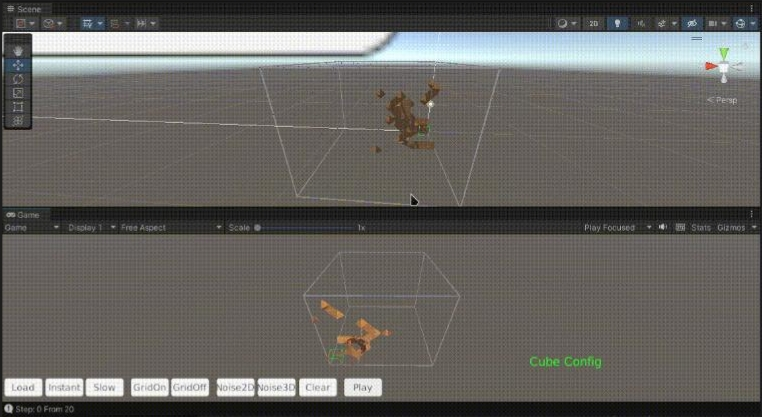
\includegraphics[width=0.9\textwidth]{tumor.jpg}
  \caption{An example of simulating tumor growth in 3D at early stages.}
\end{figure}

The creation of a tool to simulate tumor growth using cellular automaton in any organ of the human body is a significant advancement in the field of modeling and simulation of biological systems. This tool provides an innovative and flexible approach to studying tumor growth, which has important implications in both basic research and clinical applications.

The ability to load specific configurations and adjust, add, or remove parameters that influence the realism of the simulation allows for the adaptation of the model to different scenarios and conditions. This makes the tool highly versatile and applicable to a wide range of situations and types of tumors.

The use of cellular automaton in tumor growth simulation allows for the accurate representation of the interaction between cells and their environment, as well as the temporal changes that occur. This modeling approach provides a detailed understanding of tumor growth dynamics and can be used to investigate various scenarios and conditions~\cite{2}.\\

How much progress has been made so far?
\begin{itemize}
    \item The loading and usage of parameters for the simulation have been implemented.
    \item The engine to simulate the growth of a tumor in small organs has been implemented.
    \item The cell graph with its connections has been visualized and analyzed.
    \item The size that the tumor will take during the simulation has been visualized.
\end{itemize}

What will be the focus in the next stages? 
\begin{itemize}
    \item Improving all of the above, for example, enhancing the implementation of 3D rendering using Marching Cubes to obtain smoother faces and triangles.
    \item Implementing changes between states following the details found in the literature.
    \item Implementing efficient algorithms to process large amounts of cells and their connections, we are talking about millions of both.
    \item Add Artificial Intelligence and Machine Learning techniques to obtain better approximations to reality.
\end{itemize}

Finally, the 3D visualization of tumor growth using the Marching Cubes technique can provide a valuable tool for healthcare professionals to better understand the dynamics of tumor growth and develop more effective treatment strategies.

\section*{Acknowledgments}

R.R.R thanks EDITAL UFF PROPPI No. 05/2022 and PPG-MCCT of Universidade Federal Fluminense, Brazil.  P.R.B thanks CAPES, CNPq, FAPERJ, and UFF.

%%%%%%%%%%%%%%%%%%%%%%%%%%%%%
%%%%%%%%%%%%%%%%%%%%%%%%%%%%%

\section*{References}
\label{Nada}
\begin{flushleft}

\begin{thebibliography}{99}

\bibitem{1} Cirne, M. A.; Pedrini, H. Marching cubes technique for volumetric visualization accelerated with graphics processing units. Journal of the Brazilian Computer Society, vol. 19, pages 223-233, 2013. Available at: https://journal-bcs.springeropen.com/articles/10.1007/s13173-012-0097-z.

\vskip 0.2cm
\bibitem{2} Deutsch, A.; Maini, P.; Dormann, S. Cellular Automaton Modeling of Biological Pattern Formation: Characterization, Applications, and Analysis. \textit{Modeling and Simulation in Science, Engineering and Technology}. Birkhauser Boston, 2007.

\vskip 0.2cm
\bibitem{3} Guinot, V. Modelling using stochastic, finite state cellular automata: rule inference from continuum models. \textit{Applied Mathematical Modelling}, 26:701–714, 2002.


\vskip 0.2cm
\bibitem{4} Kansal, A.; Torquato, S. Simulated brain tumor growth dynamics using a three-dimensional cellular automaton. \textit{Journal of Theoretical Biology}, 203:367–382, 2000.

\vskip 0.2cm
\bibitem{5} LORENSEN, W. E.; CLINE, H. E. Marching cubes: A high-resolution 3D surface construction algorithm. ACM SIGGRAPH Computer Graphics, vol. 21, no. 4, pp. 163-169, 1987. Available at: https://people.eecs.berkeley.edu/~jrs/meshpapers/LorensenCline.pdf.

\vskip 0.2cm
\bibitem{6} Ruanxiaogang, H. A simple cellular automaton model for tumor-immunity system. In \textit{Robotics, Intelligent Systems and Signal Processing, 2003. Proceedings. 2003 IEEE International Conference on}, 2.

\vskip 0.2cm
\bibitem{7} Viera Barredo, D. Universidad de La Habana, Facultad de Matemática y Computación. Departamento de Matemática. Asesores: Reinaldo Rodríguez Ramos, Rubén Interián, Ariel Ramírez Torres, Rocío Rodríguez Sánchez. Undergraduate thesis. June, 2019.

\vskip 0.2cm
\bibitem{8} Visutsak, P. Marching Cubes and Histogram Pyramids for 3D Medical Visualization. Journal of Imaging, vol. 6, 2020. Available at: https://ncbi.nlm.nih.gov/pmc/articles/PMC8321043 and https://api.semanticscholar.org/CorpusID:225446991.

\vskip 0.2cm
\bibitem{9} Watts, D. J. \& Strogatz, S. H. Collective dynamics of small-world networks. \textit{Nature}, 393:440–442, 1998.

\end{thebibliography}

%Livro com até 3 autores:

\end{flushleft}

\end{document}
